


\section{Introduction}
	In perovskite solar cells, the absorber is usually sandwiched between two different contacts: the \acr{htm} and the \gls{etm}, with the role of extracting respectively the positive and negative free charges.
	Without this asymmetrical extraction of charges, the photogeneration would be of no use.
	The classical \acr{etm} from \gls{dssc}, mesoporous titania, is getting obsoleted by planar tin oxide \cite{Jiang2018}.
	On the contrary, the classical \acr{htm} from solid-state \gls{dssc}, \gls{spiro}, is still present in most of the record structures of \gls{csfamapbibr} based solar cells \cite{Saliba2016,Saliba2018}.
	The huge explorative work done for finding a better performing \acr{htm} managed to find very few good alternatives \cite{Rodriguez-Seco2018}.
	Still, even if the performances are at par with \gls{spiro}, the commercial price of these alternative \acr{htm} is still too high for wide area applications.
	A better understanding of the \gls{htm}\-/perovskite interaction is needed for pinpointing the key characteristics to be looked for in the next \acr{htm} design.
	In this chapter, the devices fabricated using four different \gls{htm} have been compared in order to find a correlation with the \gls{htm}'s chemical properties.
	Specifically we looked for the influence of the \acr{htm} on the device \gls{voc}.
	For \gls{osc}, the correlation between the built-in voltage and the \gls{voc} is well established \cite{Kooistra2007,Gadisa2004,Brabec2001,Wilke2012,Chen2009,Tress2011,Sanchez-Diaz2010}.
	For perovskite solar cells, some authors observed a weak correlation between the \acr{htm} ionization potential and the cell voltage \cite{Polander2014,Abate2015a,Kwon2014,Rakstys2015,Wu2016a} while others suggested a complex interplay of factors where the \acr{htm} \acr{homo} just plays a marginal role \cite{Correa-Baena2017,Belisle2016,Ishida2016,Park2018,Jimenez-Lopez2017,Tress2017}.
	The tested \acr{htm} were: the classic \gls{spiro} (\cref{fig:tae-molecules-spiro}), the previously reported \gls{tae1}\index{TAE-1} (CAS 1802982-22-4, \cref{fig:tae-molecules-tae1}, after the first report in \cite{Cabau2015a}, it has been used also by other research groups in \cite{Choi2015b,Labban2016,Wu2016a,Wu2016b}) and two novel molecules: \glsdesc{tae3} (\gls{tae3}, CAS 2055756-83-5, \cref{fig:tae-molecules-tae3}) and \glsdesc{tae4} (\gls{tae4}, \cref{fig:tae-molecules-tae4}).

	\begin{figure}
		\makebox[\textwidth][c]{
			\parbox{1.1\textwidth}{
				\centering
				\begin{subfigure}[t]{0.51\textwidth}\centering
					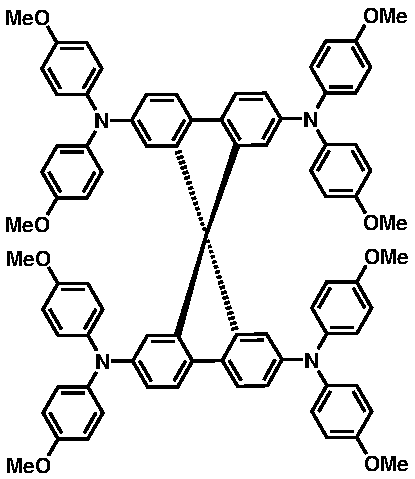
\includegraphics[scale=0.7]{molecules/spiro.pdf}
					\subcaption{\gls{spiro}}\label{fig:tae-molecules-spiro}
				\end{subfigure}
				\qquad
				\begin{subfigure}[t]{0.51\textwidth}\centering
					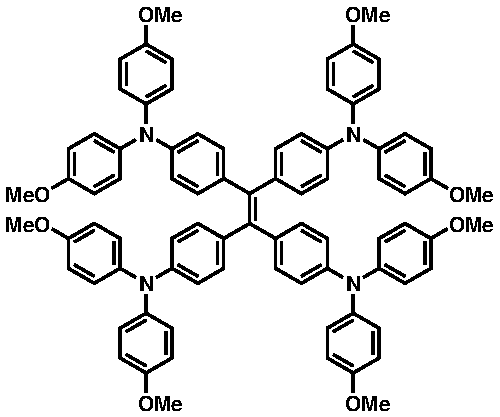
\includegraphics[scale=0.7]{molecules/tae1.pdf}
					\subcaption{\gls{tae1}}\label{fig:tae-molecules-tae1}
				\end{subfigure}
				\bigskip

				\begin{subfigure}[t]{0.51\textwidth}\centering
					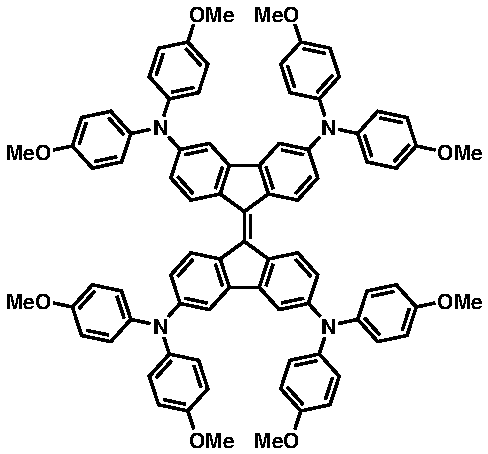
\includegraphics[scale=0.7]{molecules/tae3.pdf}
					\subcaption{\gls{tae3}}\label{fig:tae-molecules-tae3}
				\end{subfigure}
				\qquad
				\begin{subfigure}[t]{0.51\textwidth}\centering
					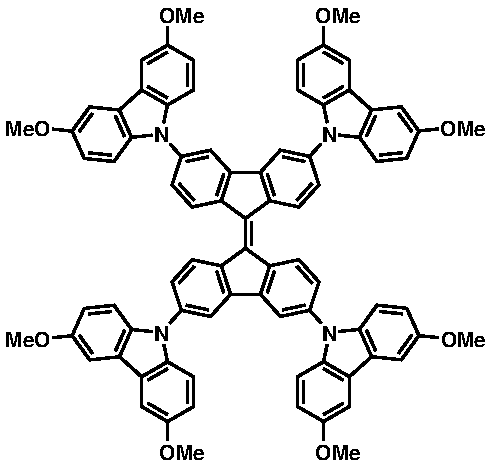
\includegraphics[scale=0.7]{molecules/tae4.pdf}
					\subcaption{\gls{tae4}}\label{fig:tae-molecules-tae4}
				\end{subfigure}
				\mycaption[Chemical structures of HTM utilised for bottom cathode solar cells.]{}\label{fig:tae-molecules}
			}
		}
	\end{figure}

	\paragraph{Design of the Experiment}
	Differently from our previous report on \gls{tae1}\index{TAE-1} \cite{Cabau2015a}, we decided to avoid the mesoporous titania layer decreasing the complexity of the stack.
	In order to compare different materials for the selective contact layer, we decided to avoid any modification to the layers underlying the absorber one in the solar cell stack, as these could heavily affect the perovskite crystallisation and morphology \cite{Tao2017,Bi2015}.
	Additionally, the \acr{htm} under comparison have been deposited under as similar as possible conditions (partially hindered by a different solubility), employing the same additives (with the same molar ratio with the \acr{htm} concentration, we used \gls{litfsi} and \iupac{4-tert-butylpyridine}) and thicknesses.
	For reducing the possible differences in \gls{dos} width, the chosen \acr{htm} have all very similar chemical structures.


	\paragraph{Author contributions}
	The devices have been fabricated by me under the supervision of Dr.\ Nuria F.\ Montcada and Prof.\ Emilio J.\ Palomares Gil (fabrication described in \cpagerefrange{methods_bottom}{methods_bottom_end}).
	The current\hyp{}voltage sweeps characterisation was performed by me and NFM\@.
	The transient electronic characterisation was performed and analysed by me using equipment built by Dr.\ Javier Pérez Hernández.
	The electrochemical and optical characterisation (cyclic voltammetry, \gls{sclc}, absorbance in solution, photoluminescence in solution) of the molecules was performed by NFM, Dr.\ Lydia Cabau, Dr.\ Agustín Molina Ontoria, and Dr.\ Inés García\hyp{}Benito.
	These same co-authors calculated \acr{homo} energies from cyclic voltammetry and hole mobilities from \gls{sclc}.
	Optical band gaps was calculated by me from absorbance in solution.
	Molecular simulations have been performed by Prof.\ Anton Vidal\hyp{}Ferran.
	Dr.\ Agustín Molina Ontoria and Prof.\ Nazario Martín designed \gls{tae1}, \gls{tae3}, and \gls{tae4}\index{TAE-4} molecules.
	The synthesis of these has been carried on by Dr.\ Inés García\hyp{}Benito and reported in her PhD thesis \cite{Garcia-Benito2017} (there, \gls{tae3}\index{TAE-3} is labelled as BF-1, and \gls{tae4}\index{TAE-4} as BF-2) and in \cite{Gelmetti2019}.
	\Gls{kpfm} measurements has been performed and interpreted by Dr.\ Ana Pérez-Rodríguez, Dr.\ Esther Barrena, and Prof.\ Carmen Ocal at ICMAB-CSIC, UAB, Barcelona.


\section{Molecular Characterisation}

	\begin{table}%[h]	% longtables cannot stay inside a float, otherwise they will not break
		\begin{xltabular}[c]{1.05\linewidth}{@{} >{\hsize=1.5\hsize}Y | >{\hsize=1.5\hsize}Y >{\hsize=0.7\hsize}Y >{\hsize=0.7\hsize}Y >{\hsize=0.9\hsize}Y >{\hsize=0.9\hsize}Y >{\hsize=0.9\hsize}Y >{\hsize=0.9\hsize}Y Y @{}}
			% multirow does not get the correct number of rows with tabularx
			% mycaption does not work inside xltabular
			\caption[Molecular properties of tested HTM.]{\textbf{Molecular properties of tested HTM.}
				The values for \gls{spiro} and for \gls{tae1}\index{TAE-1} were taken from our previous publication \cite{Cabau2015a}.
				Hole mobilities $\mu_|h|$ have been measured using \gls{sclc} fitted with Mott-Gurney law.
				$E^{\mathrm{abs}}_|onset|$ is the direct optical band gap obtained \textsl{via} Tauc plot.
				$E^{\mathrm{pl}}_|max|$ indicates the energy of the emission peak obtained exciting at \SI{550}{\nm} a solution of the molecule in \gls{thf}.
				$E^{\mathrm{exp}}_|HOMO|$ is obtained from the cyclic voltammetry of the molecules dissolved in \gls{dcm} and using ferrocene as reference.
				$E^{\mathrm{exp}}_|LUMO|$ is obtained adding the direct optical band gap $E^{\mathrm{abs}}_|onset|$ to $E^{\mathrm{exp}}_|HOMO|$ except for \gls{tae1}\index{TAE-1} where the value from \cite{Cabau2015a} has been taken.
				$E^{\mathrm{sim}}_|HOMO|$ and $E^{\mathrm{sim}}_|LUMO|$ have been obtained \textsl{via} a \gls{dft} simulation.
				$E^{\mathrm{sim,abs}}_|onset|$ is the direct optical band gap obtained \textsl{via} Tauc plot of the absorbance simulated with time-dependent \gls{dft}.
			}\label{table:tae_molecular}\\[\belowcaptionskip]
			\multirow{2}{*}{\small\gls{htm}} & \small$\mu_|h|$ & \small$E^{\mathrm{abs}}_|onset|$ & \small$E^{\mathrm{pl}}_|max|$ & \small$E^{\mathrm{exp}}_|HOMO|$ & \small$E^{\mathrm{exp}}_|LUMO|$ & \small$E^{\mathrm{sim}}_|HOMO|$ & \small$E^{\mathrm{sim}}_|LUMO|$ & \small$E^{\mathrm{sim,abs}}_|onset|$ \\
			\rule[-1ex]{0pt}{2.5ex}
			& \footnotesize\si{\square\cm\per\V\per\s} & \footnotesize\si{\eV} & \footnotesize\si{\eV} & \footnotesize\si{\eV} & \footnotesize\si{\eV} & \footnotesize\si{\eV} & \footnotesize\si{\eV} & \footnotesize\si{\eV} \\[1mm]
			\hline
			\endfirsthead
			\multicolumn{2}{@{}l}{\ldots \small continues}\\
			\hline
			\small\gls{htm} & \small$\mu_|h|$ & \small$E^{\mathrm{abs}}_|onset|$ & \small$E^{\mathrm{pl}}_|max|$ & \small$E^{\mathrm{exp}}_|HOMO|$ & \small$E^{\mathrm{exp}}_|LUMO|$ & \small$E^{\mathrm{sim}}_|HOMO|$ & \small$E^{\mathrm{sim}}_|LUMO|$ & \small$E^{\mathrm{sim,abs}}_|onset|$\\
			\hline
			\endhead
			\hline
			\multicolumn{9}{r@{}}{\small continues\ldots}\\
			\endfoot
			\hline
			\endlastfoot
			\rule[-1ex]{0pt}{3ex}
			spiro-OMeTAD 		& \num{2.6E-4} 	& 				& 					& \num{-5.10}	& \num{-2.09}	& 				&  				& \\
			TAE-1				& \num{5.9E-5} 	& \num{2.813}	& 					& \num{-5.32}	& \num{-2.74}	& \num{-5.61}	& \num{-0.54}	& \num{3.04} \\
			TAE-3 				& \num{8E-4} 	& \num{1.836}	& \num{1.722}		& \num{-5.00}	& \num{-3.16}	& \num{-5.54}	& \num{-1.77}	& \num{2.02} \\
			TAE-4 				& \num{7E-4} 	& \num{1.969}	& \num{1.771}		& \num{-5.53}	& \num{-3.56}	& \num{-6.14}	& \num{-2.27}	& \num{2.20} \\
		\end{xltabular}
	\end{table}

	\paragraph{\Glsentryshort{homo} from cyclic voltammetry}
	The oxidation potential of each \acr{htm} has been measured \textsl{via} cyclic voltammetry in solution.
	Then the energy of \acr{homo}, reported in \cref{table:tae_molecular} and represented in \cref{fig:tae-energy_levels}, has been obtained from the oxidation potential \textsl{via} the empirical linear relationship reported in \authoryear{DAndrade2005}.
	The obtained \acr{homo} value is shallowest for \gls{tae3}, then \gls{spiro} a bit above \gls{tae1}\index{TAE-1} level, and finally \gls{tae4}\index{TAE-4} being the deepest.
	Considering that these \acr{htm} gets doped by exposing the devices to dry air (see fabrication method in \cpageref{methods_bottom}, we did not add any chemical oxidiser, hopefully oxygen is enough for doping all the \acr{htm} even if their oxidation potential is quite variate), the Fermi level in these \textit{p}-type materials should be rather close to the \acr{homo}.
	The built-in voltage is defined in equilibrium as the Fermi level difference at the metallic electrodes in a complete device $V_|BI| = (\bar\mu^{\mathrm{cathode}} - \bar\mu^{\mathrm{anode}})/q$ and can be approximated by the difference in Fermi levels of the isolated \acr{etm} (which is \ch{TiO2} in all cases) and \acr{htm} $V_|BI| \approx (\bar\mu^{\mathrm{ETM}} - \bar\mu^{\mathrm{HTM}})/q$.
	So, we expect the built-in voltage to follow the trend in $\bar\mu^{\mathrm{HTM}}$ and to be larger for the devices with \gls{tae4}\index{TAE-4} and smallest for the \gls{tae3}\index{TAE-3} ones.
	Please note that the value obtained from cyclic voltammetry in solution could be different from the \acr{homo} energy in solid state film.
	This is expected to happen due to the different permittivity of the medium (\textsl{e.g.}\ the polarization of the surroundings can stabilise the cationic state), a different strain in solid state \cite{Wei2012a}, intermolecular interactions \cite{Kashimoto2018}, and an increased order \cite{Shao2016}.
	Moreover, some chemical reactivity \cite{Carrillo2016,Kim2016a}, de-doping \cite{Kim2017}, or intermixing \cite{Domanski2016} could happen with the perovskite layer or the metallic electrode.

	\begin{SCfigure}
		\centering
		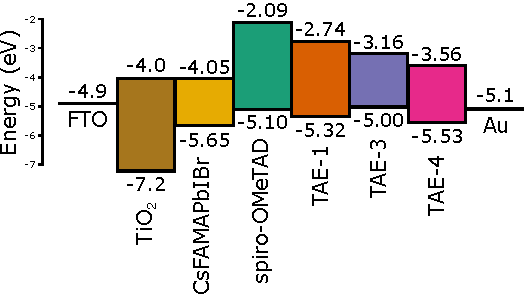
\includegraphics[width=0.7\textwidth]{energy_levels/energy_levels.pdf}
		\mycaption[Representation of HOMO and LUMO energies for the materials composing the studied cells.]{
			The \acr{homo} energy has been estimated from the oxidation potential obtained \textsl{via} cyclic voltammetry and the direct optical band gap from a Tauc plot, as described in the text.
		}\label{fig:tae-energy_levels}
	\end{SCfigure}

	\paragraph{Direct optical band gap}
	We extracted the direct band gap value from the direct Tauc plot of the absorbance onset \cite{WikipediaTauc}, an easy technique developed for crystalline and amorphous semiconductors \cite{Stenzel2005} with delocalised orbitals but often employed also for small molecules.
	A closely related value can be obtained from the photoluminescence peak maximum, which is also reported in \cref{table:tae_molecular} (but should not be used for estimating the band gap as the emission could happen from localised states with different energetics).
	The shape of the absorbance onset of an \gls{htm}, additionally to provide information on its optical band gap, can reveal the presence of mid-gap states (observable as an exponential Urbach tail) which would favour the surface recombination \cite{Tvingstedt2017}.

	\paragraph{\Glsentryshort{lumo} and selectivity}
	The optical band gap has been employed for obtaining the \acr{lumo} values reported in \cref{table:tae_molecular} and represented in \cref{fig:tae-energy_levels}.
	The selectivity of \acr{htm} has been reported to be key for perovskite solar cells' \gls{voc} \cite{Stolterfoht2018a}.
	The often neglected position of the \acr{htm} \acr{lumo} has been reported to be relevant for the injection of hot electrons, thus favouring their recombination in a recent preprint by \authoryear{Jimenez-Lopez2018} and in \authoryear{Droseros2019}.

	\paragraph{Simulated energy levels}
	The details of the molecular simulation are reported in the supplementary information of \cite{Gelmetti2019}, shortly: geometry and energy levels of the fundamental state were obtained with \gls{dft} performed including the solvent effect \textsl{via} Polarizable Continuum Model simulating the presence of surrounding tetrahydrofuran; then a time dependent \gls{dft} using hybrid exchange–correlation functional (CAM-B3LYP) allowed us to obtain the absorption spectrum.
	As can be seen in \cref{table:tae_molecular}, the \gls{dft} simulated $E^{\mathrm{sim}}_|HOMO|$ manages to reproduce the trend of the experimental $E^{\mathrm{exp}}_|HOMO|$, being the \gls{tae3}\index{TAE-3} the shallowest and \gls{tae4}\index{TAE-4} the deepest.
	Contrariwise, the simulated $E^{\mathrm{sim}}_|LUMO|$ values are rather distant from the experimental $E^{\mathrm{exp}}_|LUMO|$ ones, even if the trend is correctly reproduced.
	This can be understood considering that the $E^{\mathrm{sim}}_|LUMO|$ is simulated on top of the non\hyp{}excited molecule, which is the molecule with a fully occupied \acr{homo} level.
	This situation does not properly describe the final point of an excitation transition, where the \acr{homo} is not full as one electron have been promoted to \acr{lumo}.
	The energetic difference between the two described configurations is an electron\hyp{}hole interaction energy, which is the origin of the exciton binding energy described in \cpageref{intro_exciton}.
	The experimental direct optical band gap $E^{\mathrm{abs}}_|onset|$ can be fairly compared with the value $E^{\mathrm{sim,abs}}_|onset|$ obtained from the onset of a absorption spectra simulated with time\hyp{}dependent \gls{dft}.

	\paragraph{Other molecular characterisation}
	In the supplementary information of \cite{Gelmetti2019}, the full data of: space charge limited current, hydrogen and carbon nuclear magnetic resonance, thermo gravimetric analysis, differential scanning calorimetry, high resolution mass \textsl{via} MALDI-TOF spectrometry, cyclic voltammetry, infrared spectroscopy, elemental analysis, absorbance and photoluminescence in solution.

\section{Thin Films Morphological Characterisation}

	\paragraph{Atomic force microscopy}
	In order to verify that the various \acr{htm} gave an homogeneous coverage of the underlying layer, we performed alternated current \gls{afm}.
	As can be seen in \cref{fig:tae-afm}, all the layers have irregularities but seems that the coverage is complete.
	\Gls{tae4} surface is the most rough one, showing grains which could represent some degree of crystallisation.


	\begin{figure}
		\makebox[\textwidth][c]{
			\parbox{1.1\textwidth}{
				\centering
				\begin{subfigure}[t]{0.51\textwidth}
					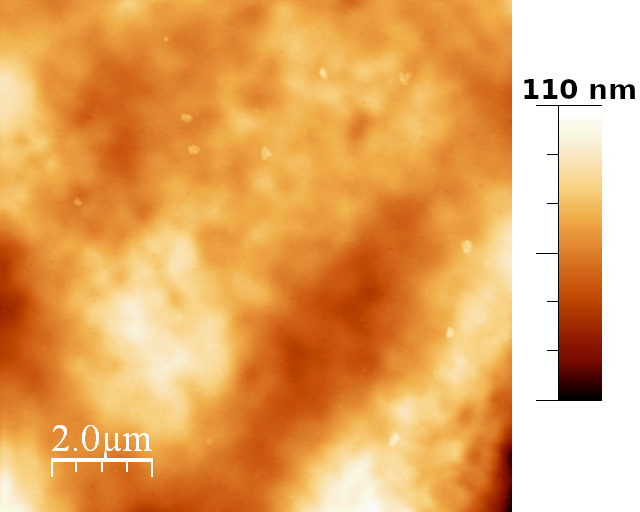
\includegraphics[width=1\textwidth]{afm/1538_spiro_190130_154619_topography.jpg}
					\subcaption{\gls{spiro}}\label{fig:tae-afm-spiro}
				\end{subfigure}
				\qquad
				\begin{subfigure}[t]{0.51\textwidth}
					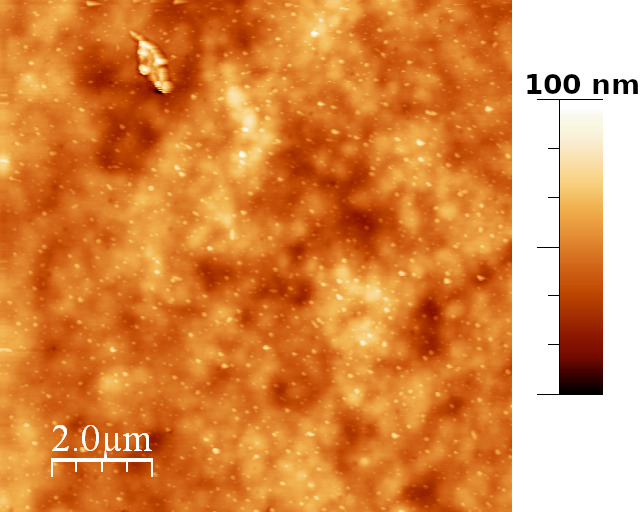
\includegraphics[width=1\textwidth]{afm/1518_tae1_190201_142020_topography.jpg}
					\subcaption{\gls{tae1}}\label{fig:tae-afm-tae1}
				\end{subfigure}
				\bigskip

				\begin{subfigure}[t]{0.51\textwidth}
					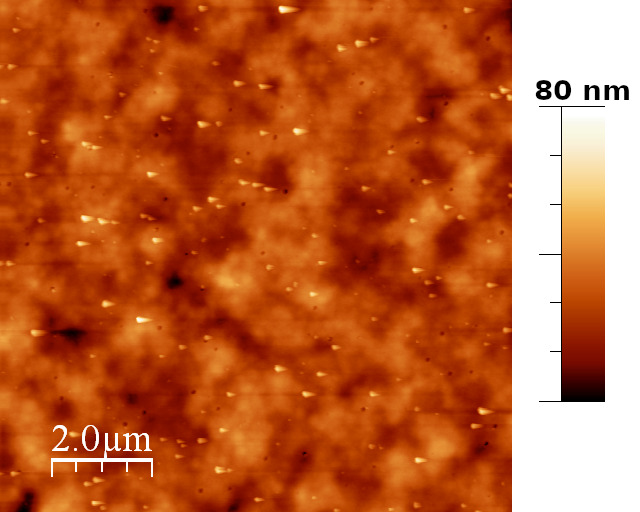
\includegraphics[width=1\textwidth]{afm/1579_tae3_190201_165210_topography.jpg}
					\subcaption{\gls{tae3}}\label{fig:tae-afm-tae3}
				\end{subfigure}
				\qquad
				\begin{subfigure}[t]{0.51\textwidth}
					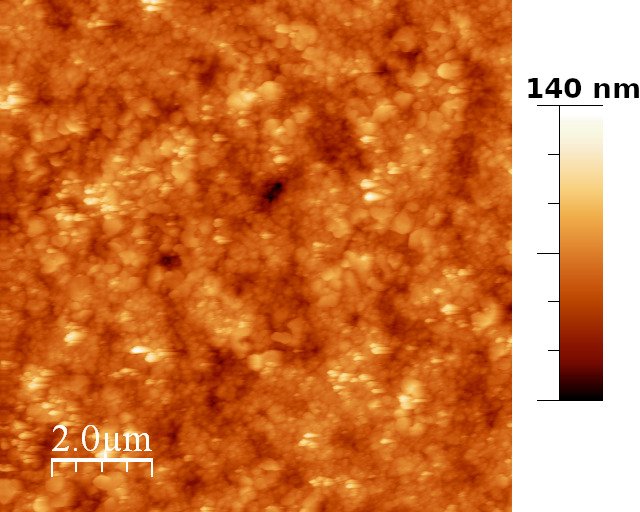
\includegraphics[width=1\textwidth]{afm/1626_tae4_190201_174638_topography.jpg}
					\subcaption{\gls{tae4}}\label{fig:tae-afm-tae4}
				\end{subfigure}
				\mycaption[Topography of HTM layered on top of perovskite, measured \textsl{via} AFM.]{
					Morphology of the surface of different \acr{htm} deposited \textsl{via} spin coating on top of \gls{csfamapbibr} perovskite layers.
					Larger scale images and phase data can be found in the supplementary information of \cite{Gelmetti2019}.
				}\label{fig:tae-afm}
			}
		}
	\end{figure}

	\paragraph{\Glsentryshort{esem} and \glsentryshort{edx}}
	The elemental analysis of the small features observed in \gls{spiro} in \cref{fig:tae-afm-spiro} were further studied with ESEM-EDX, resulting in a composition no significantly different from the rest of the surface, data in the supplementary information of \cite{Gelmetti2019}.
	In order to further assuring the complete coverage of the perovskite by the tested \gls{htm}, a cross section image has been taken for each device kind and reported in the supplementary information of \cite{Gelmetti2019}.

	\paragraph{X--Ray diffraction}
	For excluding degradation of the \gls{csfamapbibr} layer due to the contact with the \acr{htm} we performed an \gls{xrd} analysis of complete devices aged for 8 months in a nitrogen filled glovebox.
	The usage of a collimator allowed us to observe the diffraction pattern in regions not covered by the gold top electrode.
	The diffraction patterns are shown in \cref{fig:tae_xrd} and no difference can be observed between the pristine and the covered perovskite layers structure.
	Due to the penetration of the beam, also the peaks from \gls{fto} and the bump from the glass are observed.
	The patterns perfectly match the reference Cs5 pattern from \authoryear{Saliba2016}.




	\begin{figure}
		\centering
		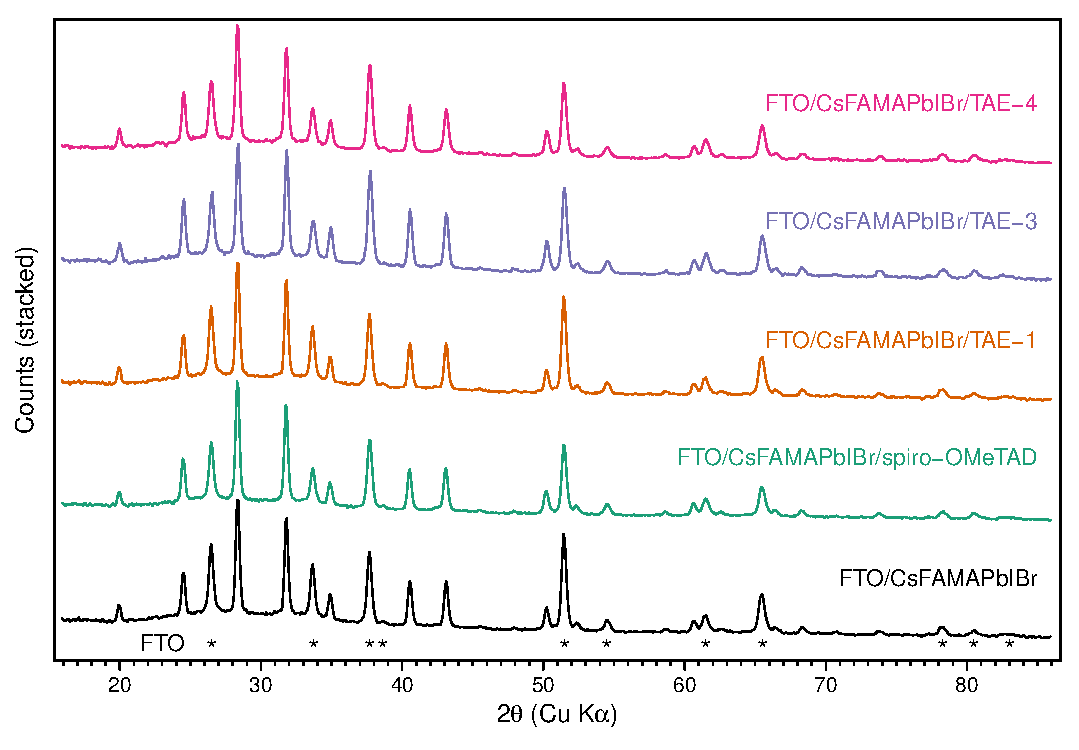
\includegraphics[width=1\textwidth]{xrd/xrd.pdf}
		\mycaption[X--Ray diffraction pattern for complete devices with different HTM.]{
			All of the patterns matches perfectly the Cs5 reference from \authoryear{Saliba2016}.
			Both the amorphous \acr{htm} and the thin \ch{TiO2} layers are not observable.
			The gold peaks are not present as the usage of a beam collimator allowe us to avoid gold covered regions.
			The peaks marked with $*$ are assigned to \gls{fto}, it can be compared with the reference PDF No.\ 00-003-1114 of \ch{SnO2}.
		}\label{fig:tae_xrd}
	\end{figure}


\section{Current-Voltage Sweeps}

	\begin{table}
		%\begin{table}%[h]	% longtables cannot stay inside a float, otherwise they will not break
		\begin{xltabular}[c]{1.05\linewidth}{@{} >{\hsize=1.4\hsize}Y| c Y Y >{\hsize=0.7\hsize}Y >{\hsize=0.9\hsize}Y @{}}
			% multirow does not get the correct number of rows with tabularx
			% mycaption does not work inside xltabular
			\caption[HTM and related average performances of bottom cathode cells.]{\textbf{HTM and related average performances of bottom cathode cells.}
				Tested \acr{htm} with \textit{average} forward and reverse J-V sweep performances.
				The standard deviation for each value is indicated after the $\pm$ symbol.
				For each reported result, at least 85, 23, 29 and 21 devices were averaged respectively for \gls{spiro}, \gls{tae1}, \gls{tae3}, and \gls{tae4}\index{TAE-4} containing solar cells.
				The measurement conditions were \SI{1}{sun} illumination, one minute light soaking, \SI{0.6}{\V\per\s} sweep speed.
				A boxplot representation of this data can be found in the supplementary information of \authoryear{Gelmetti2019}.
				J-V curve for record devices are reported in \cref{fig:tae-jv_champions}.
			}\label{table:tae_jv}\\[\belowcaptionskip]
			\multirow{3}{*}{\small\textbf{\gls{htm}}} 	& \multicolumn{5}{c}{\small\textbf{J-V sweep parameters}}
			\rule[-1ex]{0pt}{3ex} \\
			&  \small Sweep & \small\gls{jsc} &  \small\gls{voc} & \small\gls{ff} &  \small\gls{pce} \\
			\rule[-1ex]{0pt}{2.5ex}  					& / 			& \footnotesize\si{\mA\per\square\cm} &  \footnotesize\si{\V} & \footnotesize\si{\%} &  \footnotesize\si{\%} \\[1mm]
			\hline
			\endfirsthead
			\multicolumn{2}{@{}l}{\ldots \small continues}\\
			\hline
			\small\gls{htm} &\small Sweep & \small\gls{jsc} & \small\gls{voc} & \small\gls{ff} & \small\gls{pce} \\
			\hline
			\endhead
			\hline
			\multicolumn{6}{r@{}}{\small continues\ldots}\\
			\endfoot
			\hline
			\endlastfoot
			\rule[-1ex]{0pt}{4ex}
			\multirow{2}{*}{\gls{spiro}}&	fwd	&	21.2	$\pm	1.6	$ &	0.97	$\pm	0.05	$ &	60	$\pm	9	$ &	12.4	$\pm	2.4	$ \\*
			&	rev	&	21.4	$\pm	1.6	$ &	1.07	$\pm	0.06	$ &	68	$\pm	11	$ &	15.6	$\pm	3.1	$ \\[1mm]
			\hline
			\rule[-1ex]{0pt}{4ex}
			\multirow{2}{*}{\gls{tae1}}	&	fwd	&	20.1	$\pm	0.9	$ &	0.91	$\pm	0.05	$ &	50	$\pm	10	$ &	9.2	$\pm	1.6	$ \\*
			&	rev	&	20.2	$\pm	0.9	$ &	0.98	$\pm	0.03	$ &	60	$\pm	10	$ &	11.9	$\pm	2.1	$ \\[1mm]
			\hline
			\rule[-1ex]{0pt}{4ex}
			\multirow{2}{*}{\gls{tae3}}	&	fwd	&	22.4	$\pm	2.0	$ &	0.76	$\pm	0.02	$ &	63	$\pm	5	$ &	10.7	$\pm	0.9	$ \\*
			&	rev	&	22.5	$\pm	1.9	$ &	0.89	$\pm	0.04	$ &	71	$\pm	6	$ &	14.1	$\pm	1.4	$ \\[1mm]
			\hline
			\rule[-1ex]{0pt}{4ex}
			\multirow{2}{*}{\gls{tae4}}	&	fwd	&	21.0	$\pm	1.9	$ &	0.81	$\pm	0.03	$ &	54	$\pm	10	$ &	9.3	$\pm	2.5	$ \\*
			&	rev	&	21.0	$\pm	1.8	$ &	0.90	$\pm	0.05	$ &	61	$\pm	9	$ &	11.6	$\pm	2.8	$ \\[1mm]
		\end{xltabular}
	\end{table}

	As can be seen in \cref{table:tae_jv}, the most significant differences in the performances of devices when changing \acr{htm} are observed in the \gls{voc}.
	\Gls{spiro} allowed the devices to achieve the highest \gls{voc}, while \gls{tae3}\index{TAE-3} and \gls{tae4}\index{TAE-4} gave the lowest voltages.
	Some minor correlation can also be observed in the other parameters, with \gls{spiro} and \gls{tae3}\index{TAE-3} giving both slightly higher \gls{jsc} and \gls{ff}.
	For all the measured solar cells, some hysteresis\index{hysteresis} is observed in the \gls{voc} and \gls{ff}.
	Sweeps at different speeds are reported in the supplementary information of \cite{Gelmetti2019}.

	\paragraph{Ideality Factor}
	From \gls{voc} \textsl{versus} light intensity we obtained the ideality factor, following the procedure described in \cpageref{characterization_ideality}.
	The data is reported in \cite{Gelmetti2019}.
	The obtained values are 1.57 for \gls{spiro}, 1.44 for \gls{tae1}, 1.79 for \gls{tae3}, and 1.83 for \gls{tae4}.
	This data can be used for having some information on the trap level position inside band gap and on the Fermi level of the \acr{htm} \cite{Calado2019}.
	With some caution (we employed the classical method, not the improved one described in \cpageref{transient_suns_voc}) we can state that trap levels close to the mid gap are present for all of the studied \gls{htm}.


	\begin{SCfigure}
		\centering
		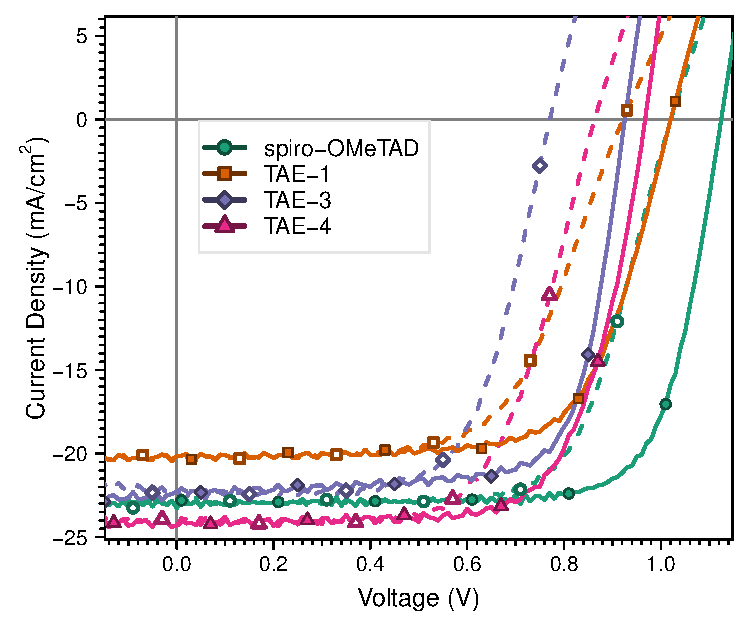
\includegraphics[width=0.8\textwidth]{jv_champions/IV-IVs.pdf}
		\mycaption[Current-voltage sweeps for champion devices with different \glsentrytext{htm}.]{The solid line with filled markers represents the forward scan, while the dashed line with hollow markers represents the reverse scan.}\label{fig:tae-jv_champions}
	\end{SCfigure}

\section{Chemical Capacitance}

	\begin{figure}
		\makebox[\textwidth][c]{
			\parbox{1.1\textwidth}{
				\centering
				\begin{subfigure}[t]{0.51\textwidth}
					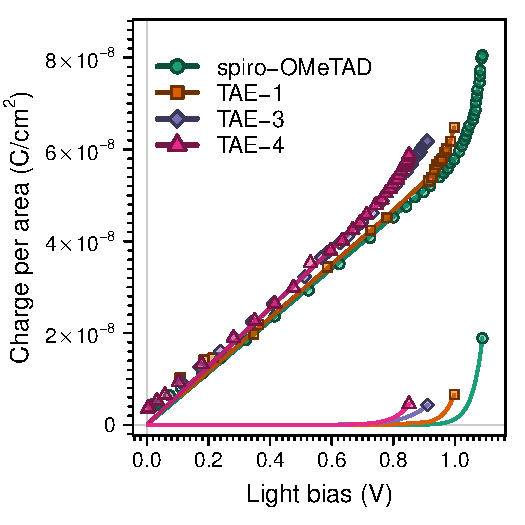
\includegraphics[width=1.05\textwidth]{photophysics/spiro_vs_TAEs-CEs.pdf}
					\subcaption{Charge from \acr{ce}}\label{fig:tae_photophysics-ce}
				\end{subfigure}
				\qquad
				\begin{subfigure}[t]{0.51\textwidth}
					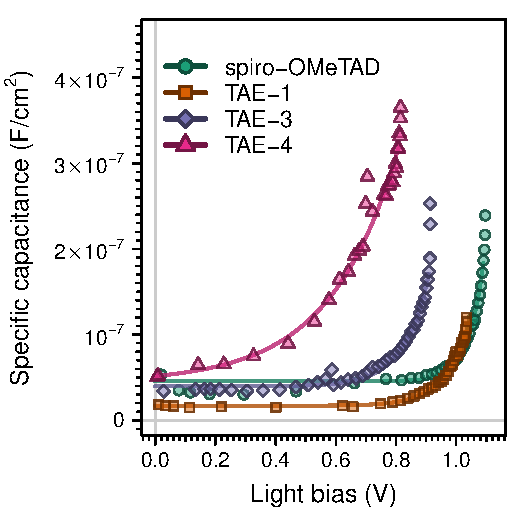
\includegraphics[width=1.05\textwidth]{photophysics/spiro_vs_TAEs-DCs-capacitance.pdf}
					\subcaption{Capacitance from \acr{dc}}\label{fig:tae_photophysics-dc}
				\end{subfigure}
				\mycaption[CE and DC of devices with different HTM, highlighting the varying chemical capacitance\index{chemical capacitance}.]{
					In (\textbf{a}) the charge \textsl{versus} light bias as obtained from \acr{ce} is reported. The dark solid line is an exponential fitting following \cref{eq:ce_full} while the light solid line is just its exponential part, ignoring the geometric capacitance\index{geometric capacitance}. In (\textbf{b}) the capacitance dependence on light bias is reported as obtained from \acr{dc}. The solid line indicates the fitting using \cref{eq:dc_full}.
				}\label{fig:tae_photophysics_cedc}
			}
		}
	\end{figure}

	Thanks to the very short measurement window (\SI{10}{\us}) we believe that no ionic displacement current\index{displacement current} (see \cpageref{intro_displacement_current} and \cpageref{ce_limitations_perovskite}) is included in our \acr{ce} experiments.
	It is interesting to compare the light bias value (open circuit voltage originated by a light intensity) at which the chemical capacitance\index{chemical capacitance} (exponential addend to the charge \textsl{versus} light bias relation, see \cpageref{ce_exp_osc}) gets relevant for the total charge.
	This growth of the chemical capacitance\index{chemical capacitance} indicates that the quasi\hyp{}Fermi levels splitting in the perovskite is approaching the built-in voltage of the device (see \cpageref{ce_energy_levels}) and can be used for estimating it.
	Both \acr{ce} and \acr{dc} show that the chemical capacitance\index{chemical capacitance} gets relevant at lower light biasses for \gls{tae4}, then \gls{tae3}, \gls{tae1}\index{TAE-1} and finally at high light bias for \gls{spiro}.
	This ordering corresponds to the one observed for the \acr{homo} energies except for the \gls{tae3}\index{TAE-3} case.
	The incoherence of the results from \acr{ce} and \acr{dc} for the \gls{tae4}\index{TAE-4} device have been confirmed on another device (not shown).
	Currently no explanation is available for explaining the deviation happening just when using this \gls{htm}.

\section{Transient Lifetime}


	As can be seen in \cref{fig:tae_photophysics_tpv}, the small perturbation lifetimes at \SI{1}{sun} illumination (for each device, the point at bottom right in the series) does not differ by much: from \SI{0.3}{\us} for \gls{spiro} to \SI{1.1}{\us} for \gls{tae4}.
	This is exactly opposed to the expected trend, where \gls{spiro} giving the best performances should have shown the longest (small perturbation) lifetimes at 1~sun which would mean less recombination.
	A much more meaningful result can be obtained referencing the small perturbation lifetimes obtained from \acr{tpv} to the chemical charge concentration (the charge stored in the perovskite layer, estimated from the exponential parts of \cref{fig:tae_photophysics_cedc}), and correcting the resulting data with the recombination order, as explained in \cpageref{characterization_tpvce}.
	This way, the data points get closer indicating very similar recombination rates at the same excess chemical charge density (vertical comparison in \cref{fig:tae_photophysics_tpvdc,fig:tae_photophysics_tpvdc} data) being present for all the cases which thus are of no help for explaining the observed \gls{voc} differences.
	The difference in lifetimes in \gls{tae4}\index{TAE-4} devices when referencing to \acr{ce} or \acr{dc} is due to the large incoherence of \acr{ce} or \acr{dc} for this device, as shown in \cref{fig:tae_photophysics_cedc}.


	\begin{table}
		\begin{xltabular}[c]{1.05\linewidth}{@{} >{\hsize=1.2\hsize}Y | >{\hsize=0.7\hsize}Y | >{\hsize=1.3\hsize}Y >{\hsize=1.3\hsize}Y >{\hsize=0.45\hsize}Y | >{\hsize=1.3\hsize}Y >{\hsize=1.3\hsize}Y >{\hsize=0.45\hsize}Y @{}}
			% multirow does not get the correct number of rows with tabularx
			% mycaption does not work inside xltabular
			\caption[Parameters fitted from TPV, TPV-CE, and TPV-DC data, from devices with different HTM.]{\textbf{Parameters fitted from TPV, TPV-CE, and TPV-DC data, from devices with different HTM.}
				The experimental data reported in \cref{fig:tae_photophysics_tpvcedc} has been fitted using \cref{eq:tpv_tau_vs_intensity} for \acr{tpv} data (using a $T$ of \SI{300}{\celsius}) and \cref{eq:tau_pfo} for \gls{tpvce} and \gls{tpvdc} data.
			}\label{table:tae_photophysics}\\[\belowcaptionskip]
			\multirow{3}{*}{\textbf{HTM}} & \textbf{\acr{tpv}} & \multicolumn{3}{c|}{\small\textbf{\gls{tpvce}}} & \multicolumn{3}{c}{\small\textbf{\gls{tpvdc}}}
			\rule[-1ex]{0pt}{3ex} \\
			& \small\gls{symb:v} & \small$k$ & \small\gls{symb:tau0} & \small\gls{symb:Phi} & \small$k$ & \small\gls{symb:tau0} & \small\gls{symb:Phi}  \\
			\rule[-1ex]{0pt}{2.5ex}   & - &  \footnotesize\si{\s^{-1}.\cm^{2\Phi-2}} & \footnotesize\si{\s}& - &  \footnotesize\si{\s^{-1}.\cm^{2\Phi-2}}& \footnotesize\si{\s} &  - \\[1mm]
			\hline
			\endfirsthead
			\multicolumn{2}{@{}l}{\ldots \small continues}\\
			\hline
			\small\gls{htm} & \small\gls{symb:v} & \small$k_|TPV-CE|$& \small$\tau_{0,\mathrm{TPV-CE}}$ & \small$\Phi_|TPV-CE|$ & \small$k_|TPV-CE|$& \small$\tau_{0,\mathrm{TPV-CE}}$ & \small$\Phi_|TPV-DC|$ \\
			\hline
			\endhead
			\hline
			\multicolumn{6}{r@{}}{\small continues\ldots}\\
			\endfoot
			\hline
			\endlastfoot
			\rule[-1ex]{0pt}{4ex}
			\gls{spiro}	& \rnum{2.07090585704198274280}	& \rsnum{.089670}							& \rsnum{1644.5868708489}	& \rnum{1.65526}	& \rsnum{.0000000012677273851307339}		& \rsnum{2383.40662630806}	& \rnum{2.39888} \\
			\gls{tae1}	& \rnum{1.69834635792333172897}	& \rsnum{.0000012125681615542155824199981}	& \rsnum{42728824.6935065}	& \rnum{2.07791}	& \rsnum{.0000000000000000000049164511186}& \rsnum{70957827.1284169}	& \rnum{3.4511} \\
			\gls{tae3}	& \rnum{2.60358060992170656706}	& \rsnum{.0034108286886881829748637047853}	& \rsnum{0.0353967580086076}& \rnum{1.7992}		& \rsnum{.0000005230964359068281862683963}& \rsnum{0.0414669507838948}& \rnum{2.1104} \\
			\gls{tae4}	& \rnum{1.21543176059352121997}	& \rsnum{.0000000000095469441207386226347}	& \rsnum{3712226.25783568}	& \rnum{2.63246}	& \rsnum{.000000000000000000000000000000000000000000000000000000000000000000000000000000002945246552214639247}& \rsnum{4623539.4194068}	& \rnum{8.3677} \\
		\end{xltabular}
	\end{table}

	\begin{figure}
		\makebox[\textwidth][c]{
			\parbox{1.1\textwidth}{
				\centering
				\begin{subfigure}[t]{1\textwidth}
					\centering
					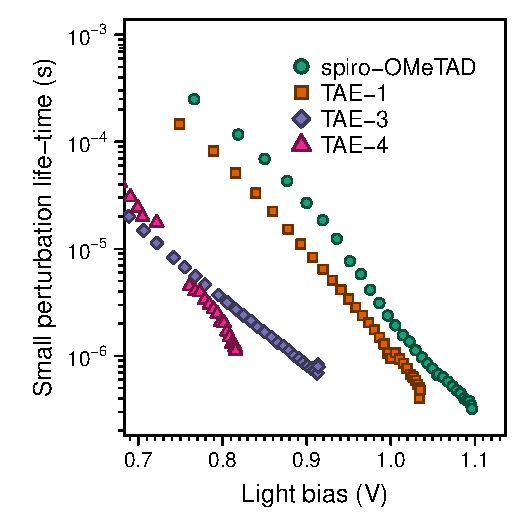
\includegraphics[width=0.51\textwidth]{photophysics/spiro_vs_TAEs-TPVs-robustmonoexp.pdf}
					\subcaption{Mono\hyp{}exponential lifetime from \acr{tpv}}\label{fig:tae_photophysics_tpv}
				\end{subfigure}
				\bigskip

				\begin{subfigure}[t]{0.51\textwidth}
					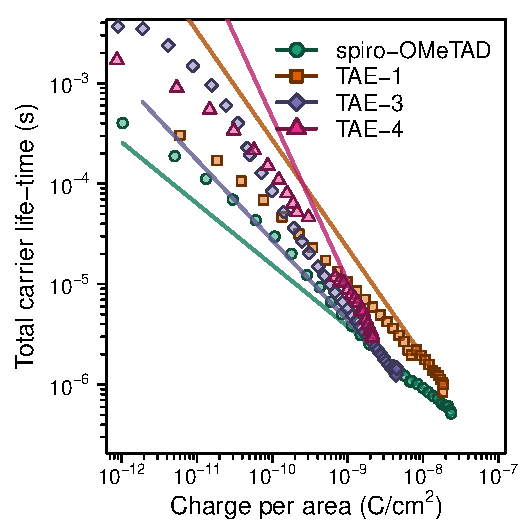
\includegraphics[width=1\textwidth]{photophysics/spiro_vs_TAEs-TPVCEs-nogeom_total.pdf}
					\subcaption{Lifetime \textsl{vs} \acr{ce} chemical charge}\label{fig:tae_photophysics_tpvce}
				\end{subfigure}
				\qquad
				\begin{subfigure}[t]{0.51\textwidth}
					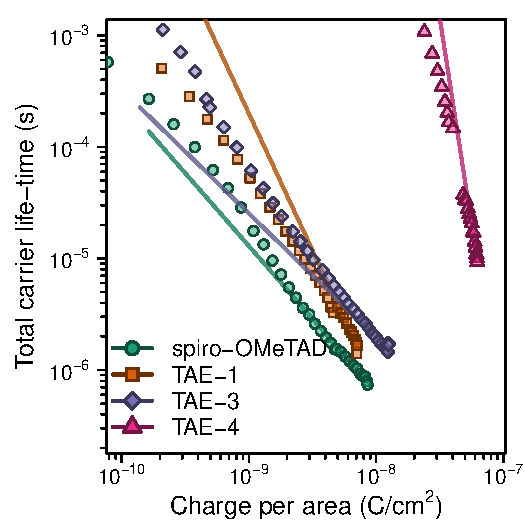
\includegraphics[width=1\textwidth]{photophysics/spiro_vs_TAEs-TPVDCs-nogeom_total.pdf}
					\subcaption{Lifetime \textsl{vs} \acr{dc} chemical charge}\label{fig:tae_photophysics_tpvdc}
				\end{subfigure}
				\mycaption[Total carrier lifetime for devices with different HTM.]{
					Four devices differing just for the employed \acr{htm} material has been compared by means of transient photophysical techniques.
					In (\textbf{a}) the plain \acr{tpv} (small perturbation lifetime \textsl{versus} light\hyp{}bias) is reported.
					In (\textbf{b}) the lifetime is plotted versus the exponential part of the charge from \acr{ce} reported in \cref{fig:tae_photophysics-ce} and corrected using \cref{eq:tau_pfo} with the recombination order obtained from the power\hyp{}law fit of the same graph.
					In (\textbf{c}) the lifetime is plotted versus the chemical charge from \acr{dc} obtained subtracting the constant geometric capacitance\index{geometric capacitance} from the data reported in \cref{fig:tae_photophysics-dc} and integrating it.
					The lifetime was corrected using \cref{eq:tau_pfo} with the recombination order obtained from the power\hyp{}law fit of the same graph.}\label{fig:tae_photophysics_tpvcedc}
			}
		}
	\end{figure}


\section{Work function of Stacked Materials}

	\begin{table}%[h]	% longtables cannot stay inside a float, otherwise they will not break
		\begin{xltabular}[c]{1.05\linewidth}{@{} >{\hsize=2\hsize}Y | Y  >{\hsize=0.9\hsize}Y >{\hsize=0.7\hsize}Y >{\hsize=0.7\hsize}Y >{\hsize=0.7\hsize}Y @{}}
			% multirow does not get the correct number of rows with tabularx
			% mycaption does not work inside xltabular
			\caption[Work function of different HTM when deposited on perovskite.]{\textbf{Work function of different HTM when deposited on perovskite.}
				The work function in \si{\eV} is reported for the surface of different \acr{htm} either deposited on top of
			}\label{table:tae_wf}\\[\belowcaptionskip]
			\multirow{3}{*}{\textbf{Substrate}} & \multirow{3}{*}{\textbf{\shortstack{Substrate\\ work\\ function}}} & \multicolumn{4}{c}{\textbf{Work function difference on top of}}
			\rule[-1ex]{0pt}{3ex} \\
			&  & \gls{spiro} & \gls{tae1}\index{TAE-1} & \gls{tae3}\index{TAE-3} & \gls{tae4}\index{TAE-4}  \\[1mm]

			\hline
			\endfirsthead
			\multicolumn{2}{@{}l}{\ldots \small continues}\\
			\hline
			Substrate	& Uncovered & \gls{spiro} & \gls{tae1}\index{TAE-1} & \gls{tae3}\index{TAE-3} & \gls{tae4}\index{TAE-4}    \\
			\hline
			\endhead
			\hline
			\multicolumn{6}{r@{}}{\small continues\ldots}\\
			\endfoot
			\hline
			\endlastfoot
			\rule[-1ex]{0pt}{4ex}
			%			\gls{fto}\-/\ch{TiO2}					&  4.81 & 4.91 &  4.85 & 5.00 & 4.92 \\
			\gls{fto}\-/\ch{TiO2}					&  $4.81$ & $+0.10$ &  $+0.04$ & $+0.19$ & $+0.11$ \\
			\hline
			\rule[-1ex]{0pt}{4ex}
			% data from received ppt
			%		\ch{TiO2}/\gls{csfamapbibr}	&  4.24 & 4.28 &  4.20 & 4.44 & 4.29  \\ 
			% data from received paper graphics
			%			\gls{fto}\-/\ch{TiO2}\-/\gls{csfamapbibr}	&  4.04 & 4.08 &  4.00 & 4.24 & 4.09  \\
			\gls{fto}\-/\ch{TiO2}/\-\gls{csfamapbibr}	&  $4.04$ & $+0.04$ &  $-0.04$ & $+0.20$ & $+0.05$  \\
		\end{xltabular}
	\end{table}

	Further characterisation of the workfunction of the \acr{htm} surface when layered on top of \gls{fto} or \ch{TiO2} or \gls{csfamapbibr} has been performed using \gls{kpfm}.
	The measured \gls{cpd} allowed us to study the impact the underlying perovskite layer can have on the \acr{htm} material.
	Perovskite Fermi level can depend on the underlying material workfunction \cite{Miller2014,Olthof2017}.
	In our case, the different values between the \gls{fto}\-/\ch{TiO2} and the \gls{fto}\-/\ch{TiO2}\-/\gls{csfamapbibr} surface workfunctions indicates that perovskite Fermi level is not pinned to the underlying layers.
	The value we observed for the \gls{csfamapbibr} surface work function matches the reported one for \gls{mapi} deposited on \ch{TiO2} \cite{Miller2014}.
	Values for \acr{htm} on top of \gls{fto}\-/\ch{TiO2} have little deviations from the value for the uncovered substrate, with the exception of \gls{tae3}.
	In the same way, the values measured for the organic layers deposited on top of \gls{fto}\-/\ch{TiO2}\-/\gls{csfamapbibr} are close to the value for the uncovered perovskite layer, also here with the exception of \gls{tae3}.
	These measurements have been discussed in Dr.\ Ana Pérez\hyp{}Rodríguez PhD thesis \cite{Perez-Rodriguez2018}.
	Within the rigid band model, the observation of such a large deviation for \gls{tae3}\index{TAE-3} indicates that the equilibrium Fermi level of the substrate is out of the \acr{htm} band gap.
	This is expected to cause a strong interfacial dipole (identifiable as depletion\index{space charge layer} layers) and a consequent vacuum level shift.

\section{Conclusions}
	Comparing the \gls{voc} obtained from solar cells having different \acr{htm} with the \acr{homo} values of these, we noticed a discrepancy.
	For understanding the origin of this incoherence, the electronic band gap was measured using \acr{ce} and \acr{dc}, which was in accordance with the observed \gls{voc} with exception of the inversion of \gls{tae3}\index{TAE-3} and \gls{tae4}\index{TAE-4} molecules order.
	This data indicates that the \acr{homo} value measured in solution \textsl{via} cyclic voltammetry is quite different from the actual energy levels for the molecules in solid thin film.
	The analysis of the total carrier lifetimes using \acr{tpv} referenced to chemical charge, has shown that the recombination rates at the same excess charge density are in the same order of magnitude regardless the employed \gls{htm}.
	The measurement of the work function of the \acr{htm} when layered on perovskite has shown the formation of a large dipole at the perovskite\-/\gls{htm} interface mainly for the \gls{tae3}\index{TAE-3} case.
	This shift in the vacuum level could be the cause for the lower \gls{voc} measured using this \acr{htm} and justify the incoherence with the observed electronic band gap in \acr{ce} and \acr{dc}.
